\documentclass[tikz]{standalone}
\begin{document}
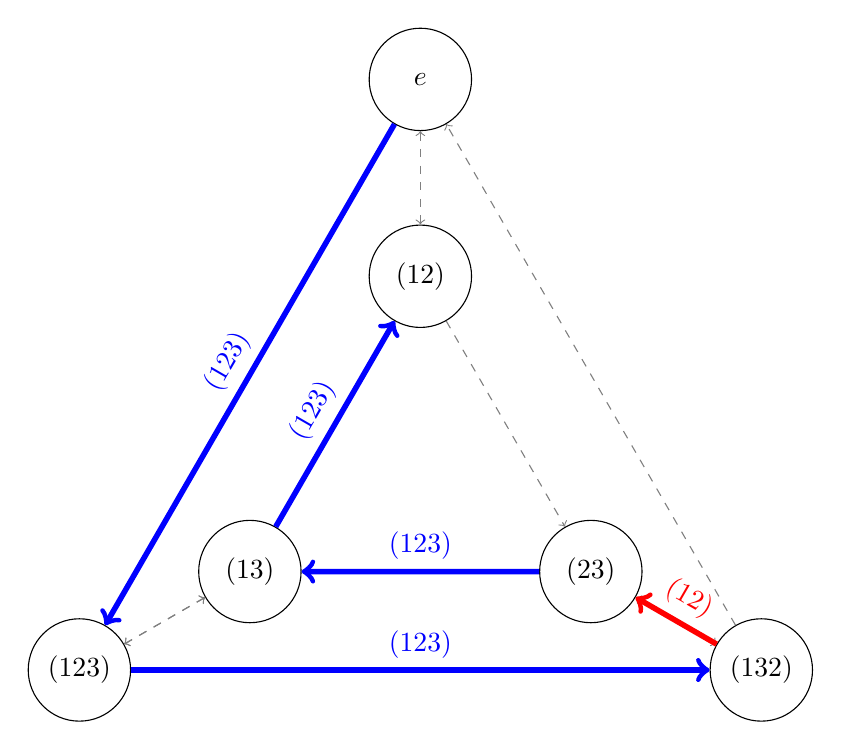
\begin{tikzpicture}[scale=2.5]
  \node[draw, circle, minimum size = 1.3cm] (e)   at (0,2)               {$e$};
  \node[draw, circle, minimum size = 1.3cm] (12)  at (0,1)               {$(12)$};
  \node[draw, circle, minimum size = 1.3cm] (123) at ({-sqrt(3)},-1)     {$(123)$};
  \node[draw, circle, minimum size = 1.3cm] (13)  at ({-sqrt(3)/2},-1/2) {$(13)$};
  \node[draw, circle, minimum size = 1.3cm] (132) at ({sqrt(3)},-1)      {$(132)$};
  \node[draw, circle, minimum size = 1.3cm] (23)  at ({sqrt(3)/2},-1/2)  {$(23)$};

  % \foreach \v in {e,12,123,13,132,23} {
  %   \foreach \w in {e,12,123,13,132,23} {
  %     \draw [thin, gray] (\v) to (\w);
  %   }
  % }
  \draw [thin, gray, dashed, <->] (e) to (12);
  \draw [thin, gray, dashed, <->] (23) to (132);
  \draw [thin, gray, dashed, <->] (13) to (123);
  \draw [thin, gray, dashed, <->] (13) to (123);
  \draw [thin, gray, dashed, ->] (12) to (23);
  \draw [thin, gray, dashed, ->] (132) to (e);
  \draw[->, line width = 0.2em, blue] (e) to node[sloped,above]{$(123)$} (123);
  \draw[->, line width = 0.2em, blue] (123) to node[sloped,above]{$(123)$} (132);
  \draw[->, line width = 0.2em, red] (132) to node[sloped,above]{$(12)$} (23);
  \draw[->, line width = 0.2em, blue] (23) to node[sloped,above]{$(123)$} (13);
  \draw[->, line width = 0.2em, blue] (13) to node[sloped,above]{$(123)$} (12);
\end{tikzpicture}
\end{document}
